\textcolor{black}{\section{Resultados y Análisis}}
\noindent (Primero muestro la gráfica y después hago el análisis de por qué hacerla loglog).

Los resultados obtenidos se muestran en la gráfica \ref{fig:1v2}

\begin{figure}[H]
	\centering
	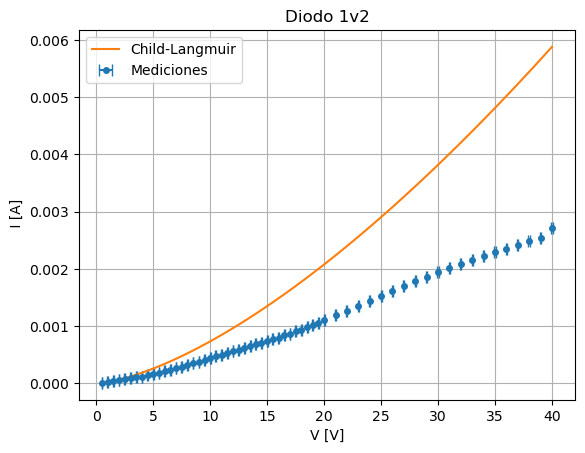
\includegraphics[scale=0.5]{figs/Diodo1v2.png}
	\caption{Datos obtenidos para los voltajes registrados. La linea continua representa el valor esperado a partir de la Ley de Child-Langmuir}
	\label{fig:1v2}
\end{figure}

Para poder obtener el cociente carga-masa del electrón, realizamos la gráfica de los datos tabulados en loglog.

\begin{figure}[H]
	\centering
	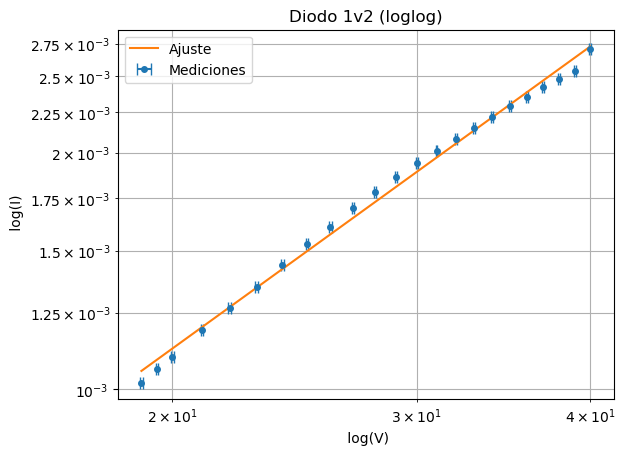
\includegraphics[scale=0.5]{figs/loglog.png}
	\caption{Gráfica loglog}
	\label{fig:logg}
\end{figure}

la relación lineal que se observa tiene una pendiente de $m = 1.276$ y una ordenada al origen $b = -10.610	$ con una desviación $rmse = 9.689$ y un coeficiente $R^2 = 0.995$

Podemos determinar a partir de la ordenada al origen $b$ la relación carga-masa pues, se sigue de la  ec. \eqref{eq:loglog} que: $\frac{e}{m_e} = (\frac{1}{B}e^{b})^{2} $. 

La razón $\frac{e}{m_e}$ obtenida experimentalmente a partir de este método es de $\frac{e}{m_e} = 1.98303463524863e11 \pm 3.842580922619109e12$ y la razón real tiene por valor: $\frac{e}{m_e} = 1.75882000837799e11$. Obteniendo un error relativo de $ E_r = -0.113$  


También podemos verificar el comportamiento potencial esperado que es $\frac{3}{2} = 1.5$  característico de la ley. La pendiente de la gráfica \ref{fig:logg} nos indica que el comportamiento del exponente calculado experimentalmente es de $1.276$, esto nos da un error relativo en el comportamiento obsrvado de $E_r = 0.149 $ con respecto a la Ley de Child-Langmuir.

\noindent
